\documentclass{article}
\usepackage[a4paper,margin=0.8in]{geometry}

\usepackage{amssymb,amsmath,amsthm,latexsym}
\usepackage{mathpartir}
\usepackage{multirow}

\usepackage{url}
\usepackage{hyperref}

% for semantic brackets
\usepackage{stmaryrd}

%% for \dblcolon
\usepackage{mathtools}

%% uses the AMS Euler math font.
\usepackage{euler}

%% for \underaccent
\usepackage{accents}

%% for colors
%% must be loaded before tikz in order for options to take effect :/
\usepackage[dvipsnames]{xcolor}

%% for drawing Hasse diagrams and commutative diagrams.
\usepackage{tikz}
\usepackage{tikz-cd}

%% for aligning tikz diagrams vertically with tables
\usepackage{adjustbox}


%% Commands
\newtheorem{theorem}{Theorem}
\newtheorem{corollary}{Corollary}
\newtheorem{conjecture}{Conjecture}
\newtheorem{lemma}{Lemma}
\newtheorem{principle}{Principle}

\newcommand{\todo}[1]{{\color{red}#1}}

\newcommand{\bnfeq}{\dblcolon=}
\newcommand{\defeq}{\overset{\ms{def}}{=}}

\newcommand{\ms}[1]{\ensuremath{\mathsf{#1}}}
\newcommand{\mb}[1]{\ensuremath{\mathbf{#1}}}
\newcommand{\mi}[1]{\ensuremath{\mathit{#1}}}
\newcommand{\mc}[1]{\ensuremath{\mathcal{#1}}}

\newcommand{\GG}{\Gamma}

\newcommand{\N}{\mathbb{N}}
\newcommand{\x}{\times}
\newcommand{\fn}{\lambda}
\newcommand{\binder}{.\,}
\newcommand{\bind}[1]{{#1}\binder}
\newcommand{\sub}[1]{\{{#1}\}}
\newcommand{\fix}{\ms{fix}}

%% TODO: get rid of \Disc, \Codisc.
\newcommand{\Disc}{{\color{red}\square}}
\newcommand{\Codisc}{{\color{red}\lozenge}}

\newcommand{\den}[1]{\llbracket{#1}\rrbracket}

%% Category & preorder theory
\newcommand{\op}{\ms{op}}
\newcommand{\iso}{\ms{iso}}
\renewcommand{\path}{\ms{path}}
\newcommand{\isoto}{\simeq}
\newcommand{\pathto}{\sim}

%% tones: mono, anti, discrete, bivariant
%% \newcommand{\tm}{{\ensuremath{1}}}     % monotone
%% \newcommand{\ta}{{\ensuremath{-1}}}    % antitone
%% \newcommand{\ti}{{\ensuremath{\bot}}} % invariant / discrete
%% \newcommand{\tb}{{\ensuremath{\top}}}  % bivariant

%% %% \renewcommand{\ti}{{\ensuremath{\star}}} % invariant / discrete
%% %% \renewcommand{\tb}{{\ensuremath{\top}}}  % bivariant

%% \renewcommand{\ti}{{\ensuremath{\square}}} % invariant / discrete
%% \renewcommand{\tb}{{\ensuremath{\lozenge}}}  % bivariant

%% \renewcommand{\tm}{{\ensuremath{+}}}   % monotone
%% \renewcommand{\ta}{{\ensuremath{-}}}   % antitone
%% %% \renewcommand{\tb}{{\ensuremath{\pm}}} % bivariant
%% %% \renewcommand{\ti}{{\ensuremath{!}}}   % invariant/discrete

\newcommand{\tm}{{\ms{id}}}     % monotone
\newcommand{\ta}{{\color{ForestGreen}\ensuremath{\op}}}    % antitone
\newcommand{\ti}{{\color{NavyBlue}\ensuremath{\iso}}} % invariant / discrete
\newcommand{\tb}{{\color{Bittersweet}\ensuremath{\path}}}  % bivariant

\newcommand{\tc}{\cdot}         % tone composition

\newcommand{\h}[3]{#1 :^{#3}\! {#2}}
\newcommand{\hm}[2]{\h{#1}{#2}{\tm}}
\newcommand{\ha}[2]{\h{#1}{#2}{\ta}}
\newcommand{\hi}[2]{\h{#1}{#2}{\ti}}
\newcommand{\hb}[2]{\h{#1}{#2}{\tb}}

\newcommand{\mto}{\overset{\tm}{\to}}
\newcommand{\ato}{\overset{\ta}{\to}}
\newcommand{\ito}{\overset{\ti}{\to}}
\newcommand{\bto}{\overset{\tb}{\to}}

\title{Tones and types}
%% \title{Tonality and inference}
%% alternate title: Tones and types
\author{Michael Robert Arntzenius}
\date{\todo{16 November 2017 -- ???}}


\begin{document}
\maketitle

\begin{mathpar}
  \begin{array}{cccl}
    \text{types} & A,B,C \vspace{0.5em}\\
    \text{terms} & M,N,O \vspace{0.5em}\\
    \text{tones}
    & s,t,u
    & \bnfeq & \tm ~|~ \ta ~|~ \tb ~|~ \ti
    \vspace{0.5em}\\
    \text{contexts}
    & \GG &\bnfeq& \cdot ~|~ \GG, \h{x}{A}{s}
    \vspace{0.5em}\\
    \text{judgment}
    & J &\bnfeq& \GG \vdash \h{M}{A}{s}
  \end{array}
\end{mathpar}

Tones represent ways a function may respect or disrespect the orderings on its
arguments. $\tm$ is monotone; $\ta$ is antitone (monotone in the
opposite ordering); $\tb$ is bivariant (monotone and antitone); and $\ti$ is
invariant (only respects equivalence).
%
Formally, tones are properties of maps between preorders (sets equipped with
reflexive, transitive relations):\,\footnote{It is possible to generalize tones
  to properties of functors and categories. In this case, invariance corresponds
  to the \emph{core} of a category, formed by throwing away all morphisms except
  the isomorphisms; while bivariance corresponds its \emph{localization}, formed
  by freely adding inverses for every morphism.}

\begin{center}
  \begin{tabular}{lclc@{\hskip 0.25em}c@{\hskip 0.25em}c}
    \multicolumn{1}{c}{\textbf{Name}}
    & \multicolumn{1}{c}{\textbf{Symbol}}
    & \multicolumn{1}{c}{\textbf{Respects}}
    & \multicolumn{3}{c}{\textbf{Property of $f$}}
    \\\hline
    \text{Monotone} & \tm
    & \text{ordering}
    & $x \le y$ &$\implies$& $f(x) \le f(y)$
    \\
    \text{Antitone} & \ta
    & \text{opposite ordering}
    & $x \ge y$ &$\implies$& $f(x) \le f(y)$
    \\
    \text{Bivariant} & \tb{}
    & \text{equivalence closure or ``paths''}
    & $x \le y \vee y \le x$ &$\implies$& $f(x) \le f(y)$
    \\
    \text{Invariant} & \ti{}
    & \text{induced equivalence or ``isomorphisms''}
    & $x \le y \wedge y \le x$ &$\implies$& $f(x) \le f(y)$
  \end{tabular}
\end{center}
In posets, antisymmetry trivializes invariance (because $x \le y \wedge y \le x
\implies x = y \implies f(x) = f(y)$), so we sometimes call $\ti$ the
``discrete'' tone, because it respects only the discrete ordering.

Another view of tones is as functors $-^s : \mb{Preorder} \to \mb{Preorder}$
which modify a preordered set's ordering without changing its elements, namely:
\[\begin{array}{r@{\hskip 0.5em}c@{\hskip 0.5em}l
  @{\hskip 2em}c@{\hskip 2em}
  l@{\hskip 0.5em}c@{\hskip 0.5em}l}
  T_\tm(A) &=& A
  %% &\text{where}& x \le_A y &\iff& x \le_A y
  \\
  T_\ta(A) &=& A^\op
  &\text{where}& x \le_{A^\op} y &\iff& y \le_A x
  \\
  T_\ti(A) &=& A^\iso
  &\text{where}& x \le_{A^\ti} y &\iff& x \le_A y \wedge y \le_A x
  \\
  T_\tb(A) &=& A^\path
  &\text{where}& x \le_{A^\path} y &\iff&
  \exists\bind{\vec{a}} a_0 = x \wedge a_n = y \wedge {}
  \\
  &&&&&& \phantom{\exists\bind{\vec{a}}}
  \forall\bind{i} a_i \le_A a_{i+1} \vee a_{i+1} \le_A a_i
\end{array}\]

These views fit together neatly. A map $f : A \overset{s}{\to} B$ with tone $s$
is the same as a monotone map $T_s(A) \to B$:
\begin{mathpar}
  {A \mto B = A \to B}
  \qquad
  {A \ato B = A^\op \to B}
  \qquad
  {A \ito B = A^\iso \to B}
  \qquad
  {A \bto B = A^\path \to B}
\end{mathpar}

%% Also of note is that each tone $s$ has a dual $\tdual{s}$ such that $T_s(A) \to
%% B = A \to T_{\tdual{s}}(B)$:
%% \[\begin{array}{c@{\hskip 2em}l}
%%     \tdual{\tm} = \tm & A \to B = A \to B\\
%%     \tdual{\ta} = \ta & A^\op \to B = A \to B^\op\\
%%     \tdual{\ti} = \tb & \Disc A \to B = A \to \Codisc B\\
%%     \tdual{\tb} = \ti & \Codisc A \to B\todo{{} = A \to \Disc B}\\
%% \end{array}\]

%% \todo{TODO: Check these! Also, doesn't this mean everything is both left- and
%%   right-adjoint to its dual? Is that possible?}


\subsection{Tone operators}

We define two operators of interest on tones:
\begin{enumerate}
\item Meet $s \wedge t$ is greatest lower bound in the lattice ordered $\ti <
  \{\tm, \ta\} < \tb$. This gives the general tone of the pairing $\langle f,
  g\rangle : A \overset{s \wedge t}{\to} B \times C$ of two functions $f : A
  \overset{s}{\to} B$ and $g : A \overset{t}{\to} C$.

\item Composition $s \tc t$ gives the general tone of a composed function $f
  \circ g : A \overset{s\tc t}{\to} C$ when $f : B \overset{s}{\to} C$ and $g :
  A \overset{t}{\to} B$; equivalently, $A^{(s\tc t)} = (A^s)^t$ for any preorder
  $A$, and $T_{s \tc t} = T_t\,T_s$ (note that the relative order of $s,t$ swaps
  in the last equation).
\end{enumerate}

These are defined by:
\begin{mathpar}
  %% "baseline=(current bounding box.center)" incantation taken from
  %% https://tex.stackexchange.com/questions/220531/how-to-align-tikzpicture-and-text-in-a-table/220543#220543
  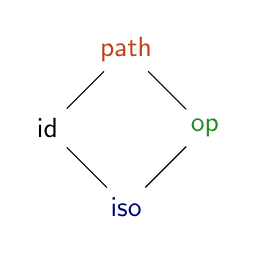
\begin{tikzpicture}[scale=1,baseline=(current bounding box.center)]
    \node (top)  at ( 0, 1) {$\tb$};
    \node (bot)  at ( 0,-1) {$\ti$};
    \node (-1)   at (-1, 0) {$\tm$};
    \node (1)    at ( 1, 0) {$\ta$};
    \draw (top) -- (-1) -- (bot) -- (1) -- (top);
  \end{tikzpicture}

  \begin{array}{c|rrrrr}
    \color{MidnightBlue} s \wedge t & \tm & \tb & \ta & \ti\\\hline
    \tm & \tm & \tm & \ti & \ti\\
    \tb & \tm & \tb & \ta & \ti\\
    \ta & \ti & \ta & \ta & \ti\\
    \ti & \ti & \ti & \ti & \ti
  \end{array}

  \begin{array}{cc|rrrr}
    \multicolumn{2}{c|}{\multirow{2}{*}{\color{MidnightBlue} $s \tc t$}}
    & \multicolumn{4}{c}{\color{MidnightBlue} t}\\
    && \tm & \ta & \ti & \tb\\\hline
    \multirow{4}{*}{\color{MidnightBlue} $s$}
    & \tm & \tm & \ta & \ti & \tb\\
    & \ta & \ta & \tm & \ti & \tb\\
    & \ti & \ti & \ti & \ti & \ti\\
    & \tb & \tb & \tb & \tb & \tb
  \end{array}
\end{mathpar}

\emph{N.B.} Monotonicity Types by Clancy, Miller, and Meiklejohn has a diagram
much like this! However, instead of bivariance they have constancy, a stricter
condition. They write $\uparrow$ for our $\tm$, $\downarrow$ for our $\ta$, $?$
for our $\ti$, and $\sim$ for constancy; they also add $=$ for the identity
function.
%%
They also have a contraction operator (``+'') on tones (``qualifiers''). I'm not
sure how or if contraction relates to tone join.

Together, $\wedge$ and $\tc$ form a semiring, with $\wedge$ as an idempotent
addition and $\tc$ as multiplication. Multiplication has $\tm$ as identity, but
lacks an absorbing zero element. (\todo{TODO: Reference ``I Got Plenty o'
  Nuttin'{}'' --- another use of variable annotations drawn from a semiring, and
  with similar (the same?) behavior of those annotations in the inference
  rules.})

The following collection of laws holds:

\begin{mathpar}
  \begin{array}{lr@{\hskip 0.5em}c@{\hskip 0.5em}l}
    \multicolumn{4}{c}{\textbf{Properties of } \wedge}
    \vspace{0.1em}\\
    \textbf{Associativity} & (s \wedge t) \wedge u &=& s \wedge (t \wedge u)\\
    \textbf{Commutativity} & s \wedge t &=& t \wedge s\\
    \textbf{Identity} & \tb \wedge s &=& s\\
    \textbf{Idempotence} & s \wedge s &=& s\\
    %% \textbf{\color{ForestGreen} Absorption} & s \wedge \ti &=& \ti
  \end{array}

  \begin{array}{lr@{\hskip 0.5em}c@{\hskip 0.5em}l}
    \multicolumn{4}{c}{\textbf{Properties of } \tc}
    \vspace{0.1em}\\
    \textbf{Associativity} & (s \tc t) \tc u &=& s \tc (t \tc u)\\
    \textbf{Identity} & \multicolumn{3}{c}{\tm \tc s = s = s \tc \tm}\\
    \ta~ \textbf{self-inverts} & \ta \tc \ta &=& \tm\\
    \tb~ \textbf{left-absorbs} & \tb \tc s &=& \tb\\
    \ti~ \textbf{left-absorbs} & \ti \tc s &=& \ti
  \end{array}

  \begin{array}{lr@{\hskip 0.5em}c@{\hskip 0.5em}l}
    \textbf{Left-distribution} & s \tc (t \wedge u) &=& (s \tc t) \wedge (s \tc u)\\
    \textbf{Right-distribution} & (s \wedge t) \tc u &=& (s \tc u) \wedge (t \tc u)
  \end{array}
\end{mathpar}

\todo{TODO: check the distribution laws hold!}


\section{A tonal sequent calculus}

These rules sent to me by Jason Reed:
\begin{mathpar}
  (A_1^{t_1}, ..., A_n^{t_n})^u = (A_1^{t_1 \tc u}, ..., A_n^{t_n \tc u})\\

  \infer[$T$-Right]{\GG \vdash A}{\GG^t \vdash T_t A}

  \infer[$T$-Left]{\GG{},A^{t\tc u} \vdash C}{\GG{}, (T_t A)^u \vdash C}

  \infer[Weakening]{\GG{}, A^t \vdash C \quad t \le u}{\GG{}, A^u \vdash C}

  \infer[Contraction]{\GG{},A^t, A^u \vdash C}{\GG{}, A^{t \wedge u} \vdash C}

  \infer[Cut]{\GG \vdash A \quad \Delta,A^t \vdash C}{\GG^t,\Delta \vdash C}
\end{mathpar}

We aim to adapt this into a natural-deduction-style system with proof terms,
i.e.\! a simply typed $\lambda$-calculus.


\section{Substitution as guiding principle}

We wish to justify some variant of the following substitution principle:

\begin{principle}[Substition]
  If $\GG_1 \vdash \h{M}{A}{s}$ and $\GG_2,\, \h{x}{A}{s} \vdash \h{N}{B}{t}$,
  then \(\GG_1 \cup \GG_2 \vdash \h{N\sub{x \mapsto M}}{B}{t}\).
\end{principle}

It's not yet clear what $\GG_1 \cup \GG_2$ should mean, exactly; \todo{we will
  return to this question.}


\section{An aside on overline notation}

An overlined and superscripted meta-expression $\overline{X}^i$ represents a
sequence (of unspecified length) with index variable $i$. The index variables
clarify which bits are repeated \emph{with variation}, and which \emph{without}.
Two examples:

\begin{center}
  \begin{tabular}{lcll}
    $\overline{x_i : A_i}^i$ & stands for
    & $x_1 : A_1,\, x_2 : A_2,\, ...,\, x_n : A_n$
    \\
    $\overline{x_i : A}^i$ & stands for
    & $x_1 : A,\hspace{0.6em} x_2 : A,\hspace{0.6em} ...,\, x_n : A$
    & ($A$ is unsubscripted, so stays the same)
  \end{tabular}
\end{center}

This is inspired by Guy Steele's talk on Computer Science Metanotation.%
%%
\footnote{There are videos of the talk at
  \href{https://www.youtube.com/watch?v=dCuZkaaou0Q}{Clojure/conj 2017} (the one
  I watched), \href{https://www.youtube.com/watch?v=7HKbjYqqPPQ}{PPoPP 2017},
  and
  \href{https://www.youtube.com/watch?v=8fCfkGFF7X8&feature=youtu.be&t=37m46s}{Harvard
    University}. There are also
  \href{http://s3.amazonaws.com/erlang-conferences-production/media/files/000/000/755/original/Guy_L._Steele_-_A_Cobbler's_Child.pdf?1510053539}{slides
    from Code Mesh 2017}.}
%%
In the talk, Guy analyses ``overline notation'' --- the use of $\overline{x}$ to
stand for a sequence $x_1, x_2, ..., x_n$.
%%
Inspired by quasiquotation in Lisp, he proposes using underlines to indicate
parts which are repeated \emph{without variation}. Thus $\overline{x : A}$
stands for $x_1 : A_1, ..., x_n : A_n$, while $\overline{x : \underline{A}}$
stands for $x_1 : A, ..., x_n : A$.
%%
In my Lisp experience, admittedly more limited than Guy's, quasiquotation is
wonderful until you need to nest it. One level of nesting is difficult to read;
two or more are unbearable. Therefore, I prefer explicit indices.


\section{Typing rules for tone synthesis}

\newcommand{\hilited}{\color{blue}}
\renewcommand{\hilited}{\color{Rhodamine}}
\renewcommand{\hilited}{\color{Emerald}}

The declarative typing rule for \textbf{let}, which internalizes the
substitution principle, is:
\begin{mathpar}
  \infer{
    \GG \vdash \h{M}{B}{s}
    \quad
    \GG, \h{x}{B}{s} \vdash \h{N}{C}{t}
  }{
    \GG \vdash \textbf{let}~ x = M ~\textbf{in}~ \h{N}{C}{t}
  }
\end{mathpar}

This can be bidirectionalized as follows, recalling that in a context, the
variables' types are inputs, but their tones are outputs:
\begin{mathpar}
  \infer{
    \overline{\h{x_i}{A_i}{\hilited s_i}}^i \vdash M \Rightarrow B
    \quad
    \overline{\h{x_i}{A_i}{\hilited t_i}}^i,\, \h{y}{B}{\hilited u}
    \vdash N : C
  }{
    \overline{\h{x_i}{A_i}{\hilited (s_i \tc u) \wedge t_i}}^i
    \vdash \textbf{let}~ y = M ~\textbf{in}~ N : C
  }
\end{mathpar}

\todo{TODO: More inference rules. E.g. pairing.}


\section{Equality of judgments at different tones}

\todo{This entire section is either outright wrong or needs much correction.}

\subsection{By example}

We hold the following judgments to be equal:
\begin{equation}\label{eqn:ex1}
 \ha{x}{A} \vdash \hm{M}{B} ~=~ \hm{x}{A} \vdash \ha{M}{B}
\end{equation}

The first judgment says the sub-expression $M$, used monotonically, will use the
variable $x$ anti-tonically. The second says that $M$, used anti-tonically, will
use the variable $x$ monotonically.

Let $f : \den{A} \to \den{B}$ be the denotation of $M$ as a single-argument
function of $x$. The first judgment says that $f$ is a monotone map from
$\den{A}$ to $\den{B}^{\op}$; the second that $f$ is monotone from
$\den{A}^{\op}$ to $\den{B}$. These amount to the same thing: $f$ is
antitone.

We also consider these judgments to be equal:
\begin{equation}
  \hm{x}{A} \vdash \hi{M}{B}
  ~=~
  \ha{x}{A} \vdash \hi{M}{B}
  ~=~
  \hb{x}{A} \vdash \hi{M}{B}
\end{equation}

This is because, when the conclusion is invariant, the only tone distinction
that matters on the variables is between invariant and everything else; any two
non-$\ti$ tones are interchangeable.

Finally, we consider these judgments to be equal:
\begin{equation} \label{eqn:ex3}
  \hb{x}{A} \vdash \hb{M}{B}
  ~=~
  \hb{x}{A} \vdash \hm{M}{B}
  ~=~
  \hb{x}{A} \vdash \ha{M}{B}
  ~=~
  \hb{x}{A} \vdash \hi{M}{B}
\end{equation}

This is because, when the hypotheses are all bivariant, the tone of the
conclusion is irrelevant.

\subsection{In general}
The general pattern which unifies equations \ref{eqn:ex1}--\ref{eqn:ex3} is:

%% TODO: remove \tdual.
\newcommand{\tdual}[1]{{\color{red}{\widehat{#1}}}}

\begin{equation}
  \overline{\h{x_i}{A_i}{\hilited s_i}}^i \vdash \h{M}{B}{\hilited \tdual{t} \tc u}
  ~=~
  \overline{\h{x_i}{A_i}{\hilited s_i \tc t}}^i
  \vdash \h{M}{B}{\hilited u}
\end{equation}

Or, perhaps more simply:
\begin{equation}
  \overline{\h{x_i}{A_i}{\hilited s_i}}^i \vdash \h{M}{B}{\hilited \tdual{t}}
  ~=~
  \overline{\h{x_i}{A_i}{\hilited s_i \tc t}}^i
  \vdash \h{M}{B}{\hilited\tm}
\end{equation}

\todo{TODO: This is wrong. In particular, $\tdual{t}$ does not in general exist.}

%% %% In Guy Steele's overline-underline notation:
%% Or, perhaps more simply:
%% \begin{equation}
%%   \overline{\h{x}{A}{\hilited s}} \vdash \h{M}{B}{\hilited t}
%%   ~=~
%%   \overline{\h{x}{A}{\hilited s \tc \underline{t}}}
%%   \vdash \h{M}{B}{\hilited\tm}
%% \end{equation}


\section{Category and preorder theory}

\[
\begin{array}{clll}
  \multicolumn{1}{l}{\textbf{Notation}}
  & \multicolumn{1}{l}{\textbf{Name}}
  & \multicolumn{1}{l}{\textbf{How to make it}}
  & \multicolumn{1}{l}{\textbf{In $\mb{Preorder}$}}
  \\\hline
  C^\path
  & \text{``localization of $C$''}
  & \text{freely add inverses for every morphism}
  & \text{equivalence closure}
  \\
  C^\iso
  & \text{``core of $C$''}
  & \text{keep only the isomorphisms}
  & \text{induced equivalence}
\end{array}
\]

$C^\path$ and $C^\iso$ are groupoids --- categories where every morphism is an
isomorphism. I assert but do not prove that $-^\path$ and $-^\iso$ are
functorial, $\mb{Cat} \to \mb{Groupoid}$. If we restrict the domain to
$\mb{Preorder}$, the codomain restricts to $\mb{Setoid}$.

Diagramatically, leaving inclusion functors unlabeled:
{\large\[
  \tikzset{
    no line/.style={draw=none,
      commutative diagrams/every label/.append style={/tikz/auto=false}}}
  \begin{tikzcd}[row sep=5em,column sep=4em]
    \mb{Cat}
    \arrow[d,bend right=40,"\textstyle\path"'{name=A}]
    \arrow[d,bend left=40,"\textstyle\iso"{name=C}]
    & \mb{Preorder}
    \arrow[d,bend right=40,"\textstyle\path"'{name=A2}]
    \arrow[d,bend left=40,"\textstyle\iso"{name=C2}]
    \arrow[l]
    \\
    \mb{Groupoid} \arrow[u,""{name=B}]
    & \mb{Setoid} \arrow{u}[name=B2]{} \arrow[l]
    %% the \dashv's between adjoint arrows
    \arrow[to path={(A) -- (B)\tikztonodes}, no line, near end]{}{\displaystyle\dashv}
    \arrow[to path={(B) -- (C)\tikztonodes}, no line]{}{\displaystyle\dashv}
    \arrow[to path={(A2) -- (B2)\tikztonodes}, no line, near end]{}{\displaystyle\dashv}
    \arrow[to path={(B2) -- (C2)\tikztonodes}, no line]{}{\displaystyle\dashv}
  \end{tikzcd}
\]}

$-^\path \dashv \mc{U} \dashv -^\iso$ form an \emph{adjoint triple}, where
$\mc{U}$ is the inclusion $\mb{Groupoid} \to \mb{Cat}$. \todo{TODO:
  Prove this, and explain what adjoint triples are.}
%
Let $\lozenge = \mc{U}(-^\path)$ and $\square = \mc{U}(-^\iso)$. This adjoint
triple implies that $\lozenge$ is a monad, $\square$ a comonad, and that
$\lozenge \dashv \square$.

Some useful notation:
\[\begin{array}{lcl@{\hskip 2em}l}
  f : x \to y : A &\iff& f \in A(x,y)
  & \text{``$f$ is an $A$-morphism from $x$ to $y$''}\\
  f : x \simeq y : A &\iff& f \in A^\iso(x,y)
  & \text{``$f$ is an $A$-isomorphism from $x$ to $y$''}\\
  f : x \pathto y : A &\iff& f \in A^\path(x,y)
  & \text{``$f$ is an $A$-path from $x$ to $y$''}
\end{array}\]

In $\mb{Preorder}$ and $\mb{Setoid}$, we can ignore the names of morphisms:
\[\begin{array}{lclcl}
  x \le y : A &\iff& \exists f \in A(x,y)\\
  x \isoto y : A &\iff& x \le y : A^\iso &\iff& x \le y \wedge y \le x : A\\
  x \pathto y : A &\iff& x \le y : A^\path
  &\iff& \exists\bind{\vec{a}} a_0 = x \wedge a_n = y
  \wedge \forall\bind{i} (a_i \le a_{i+1} \vee a_{i+1} \le a_i : A)
\end{array}\]

I may omit annotations ``$: A$'' when the intended category (groupoid, preorder,
setoid) is clear. I \emph{never} omit it in cases such as $x \le y : A^\iso$ or
$x \le y : A^\path$ --- that is, where the intended category is the result of
applying a functor.

\begin{theorem}\label{thm:loccore} For any two preorders $A$, $B$,
  \begin{equation}
    A^\path \to B = A \to B^\iso
  \end{equation}

  Where $A \to B$ is the preorder of monotone maps between $A$ and $B$.
\end{theorem}

\begin{proof} By Lemmas \ref{lem:loccore-1} and \ref{lem:loccore-2}.
\end{proof}

\begin{lemma}\label{lem:loccore-1}
  Every monotone map $A^\path \to B$ is a monotone map $A \to B^\iso$ and
  vice-versa, i.e.
  \[ \mb{Preorder}(A^\path, B) = \mb{Preorder}(A, B^\iso) \]
\end{lemma}

\begin{proof} We prove each direction:
  \begin{enumerate}
  \item Fix $F : A^\path \to B$ and suppose $x \le y : A$; we wish to show $F(x)
    \equiv F(y)$. By the definition of $A^\path$, from $x \le y$ we know $x
    \equiv y : A^\path$. Then by monotonicity of $F$ we have $F(x) \equiv F(y) :
    B$.

  \item Fix $F : A \to B^\iso$ and suppose $x \pathto y : A$; we wish to show
    $F(x) \le F(y)$. Since $x \pathto y$ there is a sequence $\vec{a}$ such that
    $a_0 = x$, $a_n = y$, and $a_i \le a_{i+1} \vee a_{i+1} \le a_i$ for $i$
    from 1 to $n-1$. From either case of this last disjunction and the
    monotonicity of $F$ we have $F(a_i) \equiv F(a_{i+1})$; by transitivity
    $F(x) \equiv F(y)$ and so $F(x) \le F(y)$.
  \end{enumerate}
\end{proof}

\begin{lemma}\label{lem:loccore-2}
  \color{red}
  \[f \le g : A^\path \to B \iff f \le g : A \to B^\iso \]

  \emph{FIXME: THIS IS WRONG! I HAVE A COUNTEREXAMPLE! Namely, $A = \{\star\}$
  and $B = \{\bot < \top\}$. Let $f(\star) = \bot$ and $g(\star) = \top$. Then
  $f \le g : A^\path \to B$ but $f \not\le g : A \to B^\iso$.}
\end{lemma}

\begin{proof}
  Expanding definitions, it suffices to show:
  \[ (\forall(a \pathto b)\ f(a) \le g(b))
  \iff
  (\forall(a \le b)\ f(a) \equiv g(b))
  \]

  We prove each direction:
  \begin{enumerate}
  \item Suppose $\forall(a \pathto b)\ f(a) \le g(b)$ and $x \le y$. From $x \le
    y$ we have $x \pathto y$ and $y \pathto x$; {\color{red} applying our first
      assumption we have $f(x) \equiv f(y)$. \emph{FIXME: This is wrong!}}

  \item Suppose $\forall(a \le b)\ f(a) \equiv g(b)$ and $x \pathto y$. We wish
    to show $f(x) \le g(y)$. Since $x \pathto y$ there is a sequence $\vec{a}$
    such that $a_0 = x$, $a_n = y$, and $a_i \le a_{i+1} \vee a_{i+1} \le a_i$
    for $i$ from 1 to $n-1$. From either case of this last disjunction and the
    monotonicity of $f : A \to B^\iso$ we have $f(a_i) \equiv f(a_{i+1})$. By
    transitivity $f(x) \equiv f(y)$, and from our first assumption and
    reflexivity $f(y) \equiv g(y)$, so transitively $f(x) \equiv g(y)$, which
    implies $f(x) \le g(y)$.
  \end{enumerate}
\end{proof}

\begin{conjecture} \label{cnj:loccore} Moreover,
  \[ A^\path \to B = {\color{ForestGreen} A^\path \to B^\iso} = A \to B^\iso \]
  because
  \[ \forall(a \pathto b)\ f(a) \equiv f(b) \]
  is equivalent to each of the conditions in lemma \ref{lem:loccore-2}.
\end{conjecture}


\begin{conjecture}
  Theorem \ref{thm:loccore} and Conjecture \ref{cnj:loccore} extend to
  categories, so that $-^\path \dashv -^\iso$ because
  \begin{equation}
    \mb{Cat}(C^\path, D) \cong \mb{Cat}(C^\path, D^\iso) \cong \mb{Cat}(C, D^\iso)
  \end{equation}
\end{conjecture}

\end{document}
